\documentclass[a4paper, openright, twoside,11pt]{article}
\usepackage[utf8]{inputenc}
\usepackage[polish]{babel}

\usepackage[T1]{fontenc}
    \usepackage{float}
    \usepackage[backend=biber, style=alphabetic, sorting=ynt]{biblatex}
    \addbibresource{biblio.bib}

    \usepackage{graphicx}
    \usepackage{romannum}
    \usepackage{amsmath}
    \usepackage{mathtools}
    \usepackage{siunitx}
    \usepackage{gensymb}
    \usepackage{amssymb}
    
    \usepackage{hyperref}
    
    \usepackage{scrlayer}
    \DeclareNewLayer[
        foreground,
        %textarea,% use only the textarea
        contents={%
          \parbox[b][\layerheight][c]{\layerwidth}
            {\centering}%
        }
      ]{blankpage.fg}
    \DeclarePageStyleByLayers{blank}{blankpage.fg}
    
    
    
    \usepackage{listings}
    \usepackage{xcolor}
    \hypersetup{
        colorlinks=false,
        pdfborder={0 0 0},
    }
    
    \usepackage{comment}
    \usepackage[normalem]{ulem}
  
   
    \usepackage[margin=1.0in]{geometry}

    
    \usepackage{fancyhdr}
    \pagestyle{fancy}
    \fancyhf{}
    \lhead{Sztuczna Inteligencja}
    \rhead{Politechnika Rzeszowska}
    \cfoot{Strona \thepage}
    %\pagenumbering{arabic}
    
    \renewcommand{\lstlistlistingname}{Spis listingów}



\begin{document}
\begin{titlepage}
            \begin{minipage}{0.3\linewidth}
                %\begin{flushleft}
                    
\includegraphics[width=1\columnwidth]{Grafika/prz_pl.png}
                %\end{flushleft}
            \end{minipage}
            \begin{minipage}{0.7\linewidth}
                \begin{center}
                    \large{Politechnika Rzeszowska\\
                    Wydział Elektrotechniki i Informatyki\\}
                    \Large\textbf{Katedra Informatyki i Automatyki}\\
                \end{center}
            \end{minipage}

            \begin{center}

                \vfill
                    \Huge Sztuczna Inteligencja\\[2cm]
                    \huge Projekt\\[2cm]
                    \huge Zrealizować sieć neuronową uczoną algorytmem wstecznej propagacji błędu z przyśpieszeniem metodą adaptacyjnego współczynnika uczenia (trainbpa) uczącą się rozpoznawania substancji odurzających.\\
                \vfill
            \end{center}



            
            
            \mbox{}
            \vfill
            \begin{flushright}
               \large{\textbf{Wykonał: \\}
               Bartłomiej Nawój\\
               156314\\
               Gr. L05 \\
                \Romannum{2} EF-DI\\[1cm]}
            \end{flushright}
            \begin{center}
                \large Rzeszów 2019
            \end{center}
        \end{titlepage}
        
    
    \newpage\null\thispagestyle{blank}\newpage
    \tableofcontents    
    \newpage\null\thispagestyle{blank}\newpage
    
    \pagenumbering{arabic}
    \newpage
    \setcounter{page}{1}
    
    \section{Wprowadzenie}
    \subsection{Cel}
    Celem projektu było stworzenie sieci neuronowej uczonej algorytmem wstecznej propagacji błędu z przyśpieszeniem metodą adaptacyjnego współczynnika uczenia, której zadaniem było rozpoznawanie substancji odurzających. Sieć została zrealizowana w programie MATLAB R2019a firmy Mathworks przy użyciu dodatku Deep Learning Toolbox.
    
    \subsection{Dane}
    Dane wykorzystywane w projekcie pochodziły z archiwum repozytorium uczenia maszynowego Uniwersytetu Kalifornijskiego w Irvine  \url{https://archive.ics.uci.edu/ml/datasets/dorothea}. Zbiór został udostępniony przez DuPont Pharmaceuticals na potrzeby konkursu KDD (Knowledge Discovery in Data Mining) Cup 2001.\\[0.5cm]
    Dorothea to zbiór danych przygotowany do przeprowadzenia testów na rozpoznawanie substancji odurzających. Związki chemiczne muszą być sklasyfikowane jako aktywne (wiążące się z trombiną), lub nieaktywne. Taka klasyfikacja umożliwia projektowanie nowych związków chemicznych, które nie tylko będą aktywne, ale również będą posiadały cechy pożądane dla leków (rozpuszczalność, brak efektów ubocznych, odpowiedni czas działania, etc.).\\[0.5cm]
    Wykorzystywany w projekcie zestaw danych to zbiór treningowy składający się z 800 przypadków, z których 78 to przypadki pozytywne (związek chemiczny sklasyfikowany jako aktywny), a 722 negatywne. Każdy z przypadków posiada 256 atrybutów. Twórcy zestawu nie zapewnili opisu atrybutów. Dane zostały znormalizowane w zakresie od -1 do +1.
    
    
    
    
    \clearpage
    \section{Opis teoretyczny}
    \subsection{Model neuronu}
   Podstawowym elementem sieci neuronowej jest sztuczny neuron. Jest to system przetwarzający wartości sygnałów na jego wejściach do jednej wartości na wyjściu. 
    \begin{figure}[h]
        \centering
        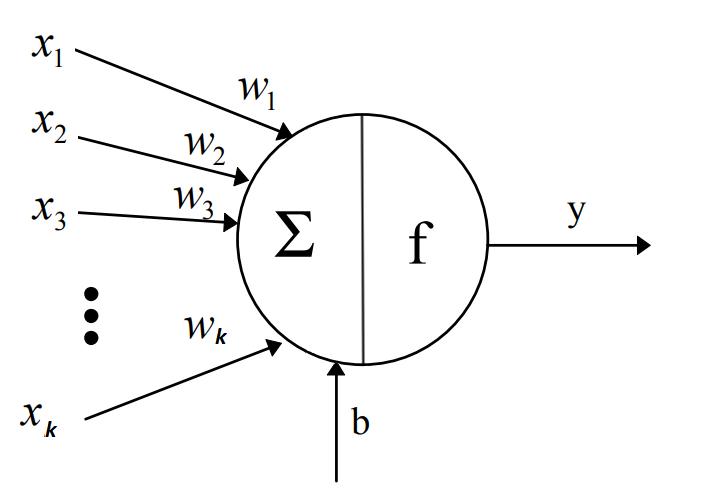
\includegraphics[width=0.6\textwidth]{Grafika/neuron.png}
        \caption{Model neuronu}
        \label{fig:neuron}
    \end{figure}\\
    gdzie:\\[0.1cm]
    $x_k$ - sygnały wejściowe\\
    $w_k$ - wagi wejść\\
    $y$ - wyjście\\
    $b$ - przesuniecie (bias)\\
    $f$ - funkcja aktywacji\\
    $k$ - liczba wejść\\
    \\[0.5cm]
    Do wyznaczenia wartości wyjścia $y$ służy wzór:
    \begin{equation}\label{fun_aktywacji}
    %y = f\left( \sum_{i=1}^k w_i x_i + b \right)
    y = f(n)
    \end{equation}
    w którym
    \begin{equation} \label{pobudzenieNeuronu}
    n = \sum_{i=1}^k w_i x_i + b
    \end{equation}
    Działanie neuronu jest następujące. Najpierw sygnały wejściowe $x_1, ...,x_k$ zostają pomnożone przez odpowiadające im wagi $w_1, ...,w_k$. Otrzymane wartości są następnie zsumowane. Dodatkowo dodawana jest wartość przesunięcia. W wyniku powstaje sygnał $n$ (nazywany łącznym pobudzeniem neuronu), który odzwierciedla działanie części liniowej neuronu. Sygnał ten jest poddawany działaniu funkcji aktywacji. W projekcie zastosowano sieć jednokierunkową, czyli taką w której nie występuje sprzężenie zwrotne.

    \clearpage
    \subsection{Sieć neuronowa}
    Neurony można łączyć w warstwy, a następnie warstwy te łączyć z innymi. Struktury zbudowane z wielu neuronów nazywamy sieciami neuronowymi. Inspiracją dla takiej struktury była budowa neuronów ludzkiego mózgu, łączących je synaps, oraz układów nerwowych. Rozpoznajemy kilka typów sieci neuronowych: jednokierunkowe, rekurencyjne, radialne i inne. Cechą wspólną wszystkich sieci neuronowych jest to, że w ich skład wchodzą połączone ze sobą neurony. Z połączeniami (synapsami) związane są wagi, których interpretacja zależy od modelu sieci.
    
    \subsection{Sieć jednokierunkowa jednowarstwowa}
    Sieć jednokierunkowa jednowarstwowa jest podstawowym elementem sieci wielowarstwowej. Neurony w tej sieci ułożone są w jednej warstwie. Przepływ sygnałów jest jednokierunkowy, tj. od wejścia do wyjścia. Każde wejście jest połączone z każdym neuronem. Dodatkowo każde z połączeń posiada własną wagę. Schemat takiej sieci przedstawiono na poniższym rysunku:
    \begin{figure}[h]
        \centering
        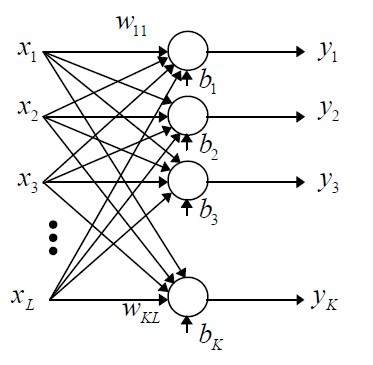
\includegraphics[width=0.5\textwidth]{Grafika/schemat_1.jpg}
        \caption{Schemat sieci jednokierunkowej jednowarstwowej}
        \label{fig:SchematSieci1}
    \end{figure}\\
    Stosując zapis macierzowy działanie warstwy neuronów można opisać wzorem:
    \begin{equation} \label{dzialanie_jednowarstwowej}
    y = f\left(w x + b \right)
    \end{equation}
    gdzie:\\[0.3cm]
    $y = [y_1, y_2, ..., y_K]^T$  - wektor sygnałów wyjściowych \\[0.3cm]
    $x = [x_1,x_2,...,x_L]^T$ - wektor sygnałów wejściowych \\[0.3cm]
    $b = [b_1,b_2, ..., b_K]^T$ - wektor przesunięć \\[0.3cm]
    $w=\begin{bmatrix}
    w_{11} & w_{12} & w_{13} & \dots  & w_{1L} \\
    w_{21} & w_{22} & w_{23} & \dots  & w_{2L} \\
    \vdots & \vdots & \vdots & \ddots & \vdots \\
    w_{K1} & w_{K2} & w_{K3} & \dots  & w_{KL}
    \end{bmatrix}$ - macierz wag
    
    \clearpage
    \subsection{Uczenie pod nadzorem pojedynczej warstwy neuronów}
    Celem uczenia pod nadzorem jest takie dobranie wag, które pozwoli na odwzorowanie danych wejściowych w wyjściowe z ustaloną dokładnością. Zmiana wag odbywa się w kolejnych cyklach uczenia oznaczonych tutaj jako $t$, zwanych epokami. Dla pojedynczej $j$-tej wagi i $i$-tego neuronu może być ona opisana następującą zależnością iteracyjną:
    \begin{equation} \label{zmiana_wag}
    w_{ij}(t+1) = w_{ij}(t) + \Delta w_{ij}(t)
    \end{equation}\\
    Uczenie pod nadzorem zakłada, że każdemu wektorowi wejściowemu $x = [x_1,x_2,...,x_L]^T$ towarzyszy pożądany wektor sygnałów wyjściowych $\hat{y} = [\hat{y}_1,\hat{y}_2,...,\hat{y}_K]^T$. Parę wektorów $(x,\hat{y})$ nazywa się parą uczącą. Jeśli sieć nie jest nauczona, to sygnał $\hat{y}$ różni się od sygnału wyjściowego $y$. Błąd popełniany przez sieć dla każdego wyjścia można zapisać jako:
    \begin{equation} \label{error}
    e_i = y_i - \hat{y}_i
    \end{equation}
    Ucząc sieć dąży się do uzyskania zgodności odpowiedzi $y$ z wartościami wymaganymi $\hat{y}$, co sprowadza się do minimalizacji funkcji błędu. Najczęściej wykorzystywaną funkcja błędu jest MSE (ang. Mean Squared Error) - błąd średnio-kwadratowy. Dla wszystkich $K$ neuronów wyznacza się go jako:
    \begin{equation} \label{error2}
    E = \frac{1}{2} \sum^K_{i=1} e^2_i
    \end{equation}\\
    Z tego powodu, że $E=E(w)$ minimum może być poszukiwane metodą gradientową. Najczęściej stosowaną metodą jest metoda największego spadku, w której wektor przyrostu wag wyraża się wzorem:
    \begin{equation} \label{gradient}
    \Delta  w = - \eta \nabla E(w)
    \end{equation}
    gdzie:\\[0.3cm]
    $\nabla$ - gradient,\\[0.1cm]
    $\eta$ - współczynnik uczenia.\\[0.3cm]
    Znak minus we wzorze (\ref{gradient}) wynika z faktu, iż gradient $\nabla E$ wskazuje kierunek najszybszego wzrostu funkcji, kiedy w minimalizacji chodzi o jak najszybszy spadek, czyli kierunek odwrotny.\\
    Ograniczając rozważania tylko do $i$-tego neuronu i $j$-tej wagi otrzymamy:\\
    \begin{equation} \label{gradient2}
    \Delta  w_{ij} = - \eta \frac{\partial E}{\partial w_{ij}}
    \end{equation}\\[0.3cm]
    Biorąc pod uwagę uwikłanie zależności $E$ od $w_{ij}$ poprzez $y_i$ i $n_i$, czyli $E = E(y_i(n_i(w_{ij})))$ pochodną możemy zapisać:\\
    \begin{equation}
    \label{eq:pochodna_gradient}
    \frac{\partial E}{\partial w_{ij}} = \frac{\partial E}{\partial y_i}  \frac{\partial y_i}{\partial n_i}  \frac{\partial n_i}{\partial w_{ij}}
    \end{equation}\\
    Uwzględniając zależności (\ref{error}) i (\ref{error2}) otrzymujemy:
    \begin{equation}
    \frac{\partial E}{\partial y_i} = y_i - \hat{y}_i = e_i
    \end{equation}
    Uwzględniając zależność (\ref{pobudzenieNeuronu}):
    \begin{equation}
    \frac{\partial n_i}{\partial w_{ij}} = x_j
    \end{equation}
    Podstawiając powyższe pochodne do równania (\ref{eq:pochodna_gradient}), a otrzymane równanie do zależności (\ref{gradient2}) otrzymujemy:
    \begin{equation}
        \label{gradient_podstawione}
        \Delta  w_{ij} = - \eta \frac{\partial E}{\partial w_{ij}} = \eta (\hat{y}_i - y_i) \frac{\partial y_i}{\partial n_i} x_j
    \end{equation}
    gdzie
    $\frac{\partial y_i}{\partial n_i} = f'(n_i)$ równe jest pochodnej cząstkowej $i$-tej funkcji aktywacji po $i$-tym łącznym pobudzeniu neuronu.
    
    
    \subsection{Sieć jednokierunkowa wielowarstwowa}
    Sieć jednokierunkowa wielowarstwowa ma zwykle jedną warstwę neuronów ukrytych między warstwą wejściową, a wyjściową.
    \begin{figure}[h]
        \centering
        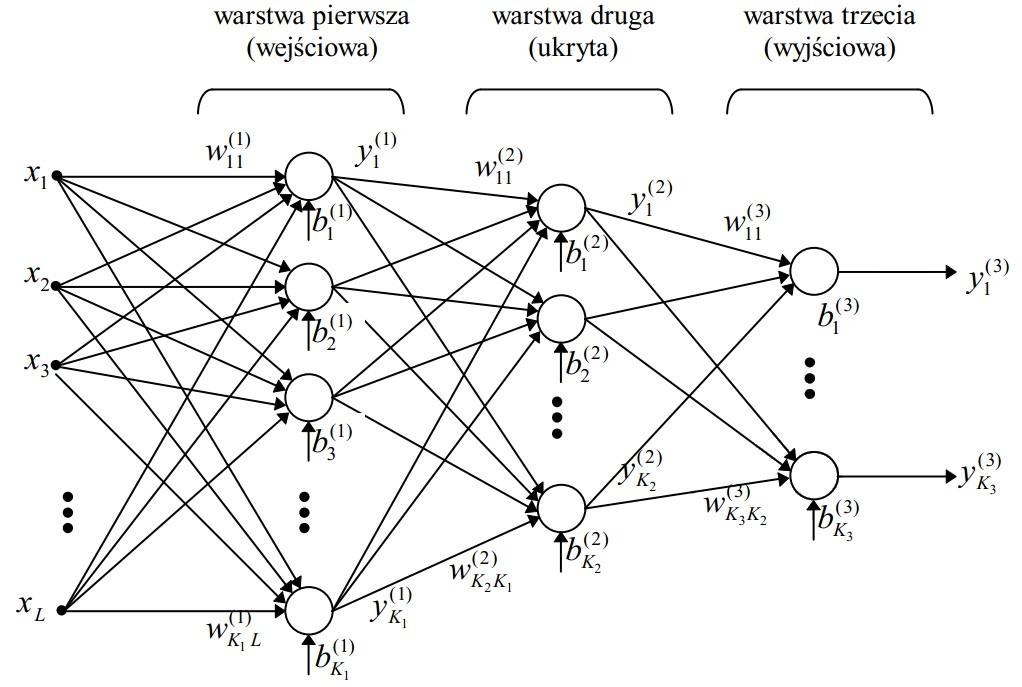
\includegraphics[width=0.8\textwidth]{Grafika/schemat_sieci.jpg}
        \caption{Schemat sieci jednokierunkowej wielowarstwowej}
        \label{fig:SchematSieci}
    \end{figure}\\
    Taką sieć nazywa się siecią trójwarstwową. Pomiędzy warstwami neuronów występują połączenia typu każdy z każdym. Sygnały wejściowe podawane są do warstwy wejściowej neuronów, których wyjścia stanowią sygnały źródłowe dla kolejnej warstwy.\\
    Każda z warstw sieci posiada własną macierz wag $w$, wektor przesunięć $b$, funkcję aktywacji $f$ oraz wektor sygnałów wyjściowych $y$. Aby możliwe było ich dalsze rozróżnianie dodano do nich numer warstwy, której dotyczą. Przykładowo dla warstwy drugiej wektor przesunięć oznaczany będzie $b^{(2)}$. Korzystając z zależności (\ref{dzialanie_jednowarstwowej}) działanie poszczególnych warstw można zapisać jako:
    
    \begin{equation}
    \begin{aligned}
    y^{(1)} &= f^{(1)}(w^{(1)}x+b^{(1)})\\
    y^{(2)} &= f^{(2)}(w^{(2)}y^{(1)}+b^{(2)})\\
    y^{(3)} &= f^{(3)}(w^{(3)}y^{(2)}+b^{(3)})\\
    \end{aligned}    
    \end{equation}\\[0.3cm]
    Działanie całej sieci z rysunku (\ref{fig:SchematSieci}) można opisać równaniem:
    \begin{equation}
    y^{(3)} = f^{(3)}\Bigg(w^{(3)}f^{(2)}\bigg(w^{(2)}f^{(1)}\Big(w^{(1)}x+b^{(1)}\Big)+b^{(2)}\bigg)+b^{(3)}\Bigg)
    \end{equation}
    
    \clearpage
    \subsection{Metoda wstecznej propagacji błędu}
    Metoda wstecznej propagacji błędu jest jedną z najczęściej stosowanych metod uczenia sieci wielowarstwowych. Jest dobrze opisana w literaturze, oraz wyróżnia się prostotą dzięki rekurencyjnemu sposobowi działania. Dla sieci z rysunku (\ref{fig:SchematSieci}) funkcja błędu (\ref{error2}) przyjmie postać:\\[0.2cm]
\begin{equation}
\begin{aligned}
    &E = \frac{1}{2} \sum_{i_{3}=1}^{K_3}e^{2}_{i_3} = \frac{1}{2}  \sum_{i_{3}=1}^{K_3}
    \Big(y^{(3)}_{i_3}-\hat y_{i_3}
    \Big)^{2} = \\
    &=\frac{1}{2}  \sum_{i_{3}=1}^{K_3}
    \Bigg( f^{(3)} 
    \Bigg(  \sum_{i_{2}=1}^{K_2}w^{(3)}_{i_3 i_2}y_{i_2}+b^{(3)}_{i_3}
    \Bigg)  -\hat y_{i_3}
    \Bigg)^{2} = \\
    &=\frac{1}{2}  \sum_{i_{3}=1}^{K_3}
    \Bigg( f^{(3)} 
    \Bigg( \sum_{i_{2}=1}^{K_2}w^{(3)}_{i_3 i_2} f^{(2)} 
    \Bigg( \sum_{i_{1}=1}^{K_1}w^{(2)}_{i_2 i_1} y_{i_1}+b^{(2)}_{i_2}
    \Bigg) +b^{(3)}_{i_3} 
    \Bigg) -\hat y_{i_3}
    \Bigg)^{2} = \\
    &=\frac{1}{2}  \sum_{i_{3}=1}^{K_3}
    \Bigg( f^{(3)} 
    \Bigg( \sum_{i_{2}=1}^{K_2}w^{(3)}_{i_3 i_2} f^{(2)}
    \Bigg( \sum_{i_{1}=1}^{K_1}w^{(2)}_{i_2 i_1} f^{(1)}
    \Bigg( \sum_{j=1}^{L}w^{(1)}_{i_1 j}x_{j} + b^{(1)}_{i_1}
    \Bigg) +b^{(2)}_{i_2}
    \Bigg) +b^{(3)}_{i_3} 
    \Bigg) -\hat y_{i_3}
    \Bigg)^{2}
\end{aligned}
\end{equation}\\
    Wyliczanie wag rozpoczyna się od wyliczenia wag neuronów warstwy wyjściowej (ostatniej). Wagi warstwy wcześniejszej obliczane są na podstawie obliczeń z warstwy ostatniej. Na podstawie tych obliczeń, wylicza się wagi warstwy poprzedzającej obie z tych warstw itd.\\
    Dla drugiej warstwy sieci z rysunku (\ref{fig:SchematSieci}) otrzymujemy:\\[0.2cm]
    \begin{equation}
    \frac{\partial E}{\partial w^{(2)}_{i_2i_1}} = \sum_{i_{3}=1}^{K_3}\Big(e_{i_3} f'^{(3)}(n_{i_3}) w^{(3)}_{i_3 i_2}\Big)
    f'^{(2)}(n_{i_2}) y^{(1)}_{i_1}
    \end{equation}\\[0.2cm]
    Analizując kolejny poziom uwikłania, dla warstwy pierwszej otrzymujemy:\\[0.2cm]
    \begin{equation}
     \frac{\partial E}{\partial w^{(1)}_{i_1j}} = f'^{(1)}(n_{i_1}) x_j 
    \sum_{i_{2}=1}^{K_2}\Bigg( f'^{(2)}(n_{i_2}) w^{(2)}_{i_2 i_1}
     \sum_{i_{3}=1}^{K_3}\bigg(e_{i_3} f'^{(3)}(n_{i_3}) w^{(3)}_{i_3 i_2}   \bigg)\Bigg)
    \end{equation}
    \clearpage
    \subsection{Adaptacyjny współczynnik uczenia}
    Metoda wstecznej propagacji błędu może być bardzo czasochłonna. Z tego powodu wymyślono szereg metod pozwalających na przyspieszenie procesu uczenia. Jedną z nich jest metoda adaptacyjnego współczynnika uczenia. Polega ona na zmienianiu współczynnika uczenia $\eta$ w odniesieniu do błędu popełnianego przez sieć. W metodzie tej błąd najczęściej wyraża się w postaci sumarycznego błędu kwadratowego $SSE$, lub błędu średnio-kwadratowego $MSE$. Wspomniane postaci błędu zapisujemy jako: \\[0.2cm]
    \begin{equation}
        SSE(t)=\sum_{i=1}^M\bigg(y_i(t)-\hat{y}_i(t)\bigg)^2
    \end{equation}\\[0.1cm]
    \begin{equation}
         MSE(t)=\frac{1}{M}\sum_{i=1}^M\bigg(y_i(t)-\hat{y}_i(t)\bigg)^2
    \end{equation}\\[0.2cm]
    Metoda polega na porównaniu błedu w chwili $t$ z poprzednią wartością. Przyjmując oznaczenie błędu jako $ERR$, zmianę współczynnika uczenia można zdefiniować jako:
    \begin{equation}
        \eta(t+1)=\begin{cases}
            \eta(t) \cdot\xi _d \qquad \qquad gdy\quad ERR(t)>er\cdot ERR(t-1)\\
            \eta(t) \cdot\xi _i \qquad \qquad gdy\quad ERR(t)<ERR(t-1)\\
            \eta(t) \qquad \quad \qquad gdy\quad ERR(t-1) \leq ERR(t)\leq er\cdot ERR(t-1)\\
        \end{cases}
    \end{equation}\\[0.2cm]
    Jeśli nowy błąd jest większy od starego błędu pomnożonego przez dopuszczalną krotność przyrostu błędu $er$ (domyślnie 1.04) nowe wagi są odrzucane, a współczynnik $\eta$ jest mnożony przez współczynnik dekrementacji $\xi _d$ (domyślnie 0.7). Jeśli zaś nowy błąd jest mniejszy niż stary, $\eta$ jest mnożony przez współczynnik inkrementacji $\xi _i$ (domyślnie 1.05).
   \clearpage
    
    
    \section{Rozwiązanie problemu}
    \subsection{Przygotowanie skryptu}
    W celu przeprowadzenia eksperymentów napisano skrypt w środowisku Matlab R2019a. W tej wersji zastąpiono funkcję $trainbpa$ funkcją $traingda$, która wchodzi w skład dodatku Deep Learning Toolbox. W algorytmie zaimplementowano 5 pętli mających na celu zbadanie następujących parametrów:
\begin{itemize}
    \item $S1$ - liczba neuronów w warstwie pierwszej
    \item $S2$ - liczba neuronów w warstwie drugiej
    \item $lr\_inc$ - wartość współczynnika inkrementacyjnego
    \item $lr\_dec$ - wartość współczynnika dekrementacyjnego
    \item $er$ - maksymalna krotność błędu
\end{itemize}
\begin{lstlisting}[language=Matlab, caption=Skrypt sieci neuronowej, label=skrypt,numbers=left]
clear;
format compact;
load dorothea2

%przygotowanie zmiennych
x = Pn;
t = T;

%Wyczyszczenie zbednych zmiennych
clearvars -except x t;

%Wektor neuronow wartswy 1 i 2
S1_vec = 10:10:100;
S2_vec = 10:10:80;

%Wektory inc/dec learning ratio i bledu
lr_inc_vec = 1.05;
lr_dec_vec = 0.7;
er_vec = 1.04;

% Zapis nagłówka dokumentu
header = 'S1\tS2\tlr_inc\tlr_dec\tmax_err\t  PK[%%]\t  lr\tMSE\t
\tepoch\twork_progress[%%]\n';
file_var = fopen('nn_logs.txt', 'wt');
fprintf(file_var, header);
formating = '%2g \t %2g \t %1.6g \t %1.6g \t %1.6g \t %3.4g 
\t %1.6g \t %4.6g \t %3.6g \t %3.6g\n';
fclose(file_var);

%zmienne do zapisu
todo = length(S1_vec)*length(S2_vec)*length(lr_inc_vec)*...
        length(lr_dec_vec)*length(er_vec);    
PK_v=zeros(length(S1_vec),length(S2_vec),length(lr_inc_vec),...
 length(lr_dec_vec),length(er_vec));
MSE_v=PK_v;
LR_v=PK_v;
EPOCH_v=PK_v;
licznik = 0;


for ind_S1=1:length(S1_vec)
    for ind_S2=1:length(S2_vec)
        for ind_lr_inc=1:length(lr_inc_vec)
            for ind_lr_dec=1:length(lr_dec_vec)
                for ind_er=1:length(er_vec)

                    licznik = licznik +1;
                    work_progress = licznik/todo *100;
                    %Utworzenie sieci
                    net = feedforwardnet([S1_vec(ind_S1),S2_vec(ind_S2)],...
                    'traingda');
                    %ustawienie wszelkich parametrow
                    net.trainParam.epochs = 20000;
                    net.trainParam.max_fail = 500;
                    net.trainParam.lr = 0.01;
                    net.trainParam.lr_inc = lr_inc_vec(ind_lr_inc);
                    net.trainParam.lr_dec = lr_dec_vec(ind_lr_dec);
                    net.trainParam.max_perf_inc = er_vec(ind_er);
                    net.trainParam.show = 100;
                    net.trainParam.showWindow = false;
                    net.trainParam.showCommandLine = true;
                    
                    %Podzial danych
                    net.divideParam.trainRatio = 80/100;
                    net.divideParam.valRatio = 10/100;
                    net.divideParam.testRatio = 10/100;

                    %trenowanie sieci
                    [net,tr] = train(net,x,t);
                    
                    %test
                    y = net(x);
                    e = t-y;
                    mse_value = immse(y,t);                    
                    PK = (1-sum(abs(t-y)>=1)/length(t))*100
                    
                    % Zapis danych do macierzy
                    PK_v(ind_S1,ind_S2,ind_lr_inc,ind_lr_dec,ind_er) = PK;
                    MSE_v(ind_S1,ind_S2,ind_lr_inc,ind_lr_dec,ind_er) = ...
                    mse_value;
                    LR_v(ind_S1, ind_S2,ind_lr_inc,ind_lr_dec,ind_er) = ...
                    net.trainParam.lr;
                    EPOCH_v(ind_S1,ind_S2,ind_lr_inc,ind_lr_dec,ind_er) = ...
                    tr.best_epoch;
                    
                     
                    % Zapis danych do pliku
                    file_var = fopen('nn_logs.txt', 'at');
                    fprintf(file_var, formating, S1_vec(ind_S1),...
                            S2_vec(ind_S2), lr_inc_vec(ind_lr_inc),...
                            lr_dec_vec(ind_lr_dec), er_vec(ind_er),...
                            PK, net.trainParam.lr, mse_value ,...
                            tr.best_epoch, work_progress);
                    fclose(file_var);
                end
            end
        end
    end
end

save("output");
% Wykresy
figure;
surf(S1_vec,S2_vec,PK_v')
xlabel('S1');
ylabel('S2');
zlabel('PK [%]');

figure;
surf(S1_vec,S2_vec,MSE_v')
xlabel('S1');
ylabel('S2');
zlabel('MSE');
\end{lstlisting}
    
    \clearpage
    \section{Eksperymenty}
    %results 05-21 10-39.mat
\subsection{Badania przesiewowe dla małej ilości neuronów}
Celem pierwszego eksperymentu było zbadanie, jaki wpływ na poprawność klasyfikacji i błąd średnio-kwadratowy ma mała liczba neuronów. W pętlach kolejno zmieniana była ilość neuronów w obu warstwach, w zakresie od 1 do 10 z krokiem 1, a następnie na podstawie uzyskanych w obliczeniach danych zostały utworzone potrzebne wykresy (listing (\ref{skrypt})).Wartości pozostałych parametrów zostały ustawione na domyślne tj. wartość współczynnika inkrementacji na $1.05$, wartość współczynnika dekrementacji na $0.7$, dopuszczalna krotność przyrostu błędu na $1.04$.

\begin{figure}[!h]
\centering
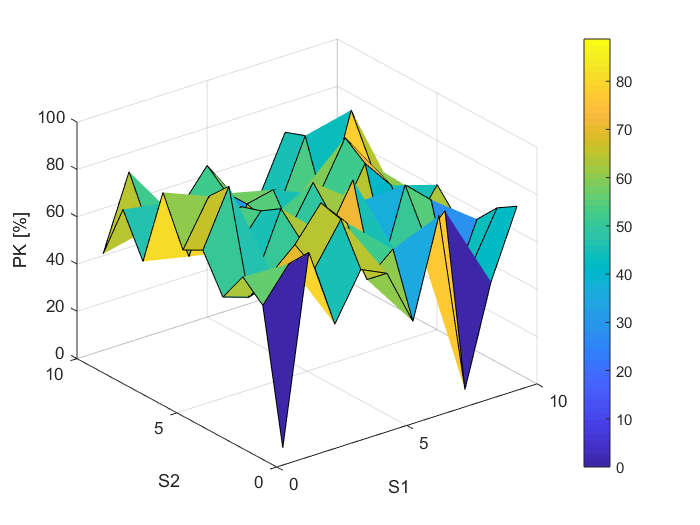
\includegraphics[width = 0.7\textwidth]{Grafika/przesiewowe_male.png}
\caption{Wpływ liczby neuronów w warstwie pierwszej i drugiej na poprawność klasyfikacji}
\label{fig:PKeksperyment1}
\end{figure}
\begin{figure}[!h]
\centering
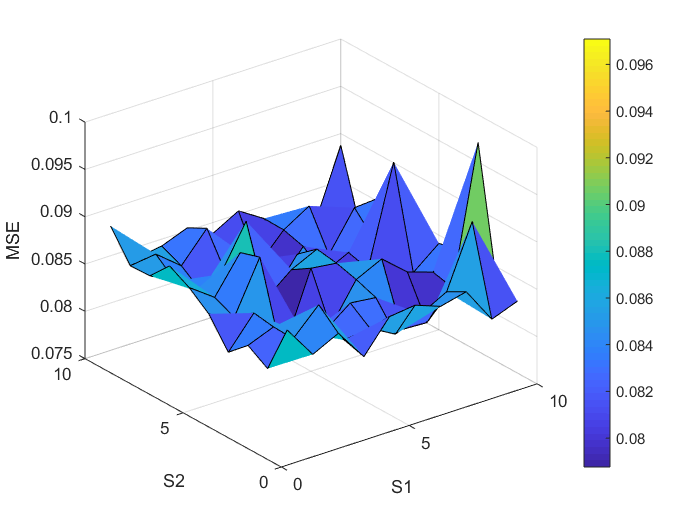
\includegraphics[width = 0.7\textwidth]{Grafika/mse_przesiewoweMale.png}
\caption{Wpływ liczby neuronów w warstwie pierwszej i drugiej na błąd średnio-kwadratowy}
\label{fig:MSEeksperyment1}
\end{figure}
\clearpage
Największą poprawność klasyfikacji ($88.75\%$) uzyskano dla 2 neuronów w warstwie pierwszej i 5 w warstwie drugiej.\\
Najmniejszy błąd średnio-kwadratowy ($0.0795748$) osiągnięty został dla 8 neuronów w warstwie pierwszej i 10 neuronów w warstwie drugiej. Dla tej konfiguracji $PK$ wyniosło $67.63\%$.





    %results 05-20 18-50.mat
\subsection{Badania przesiewowe dla dużej ilości neuronów}
Eksperyment miał na celu sprawdzenie jak zachowuje się sieć przy dużej ilości neuronów w dwóch warstwach. Wszystkie parametry pozostały bez zmian, zmieniana była jedynie ilość neuronów w zakresie od 100 do 400 z krokiem 50.
\begin{figure}[!h]
\centering
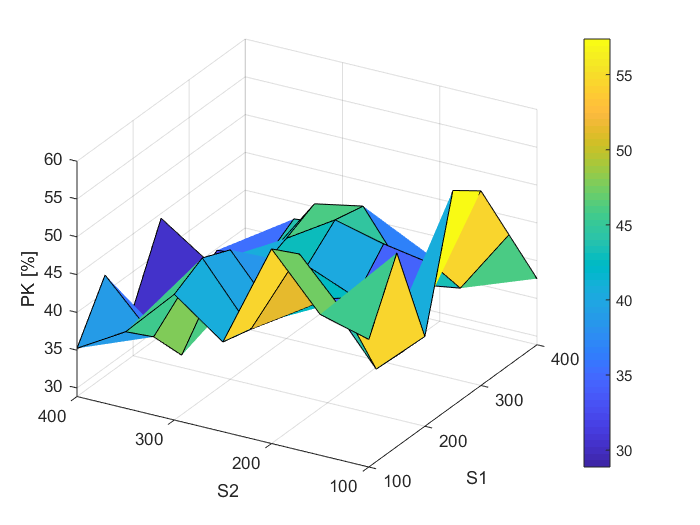
\includegraphics[width = 0.7\textwidth]{Grafika/PK_duze.png}
\caption{Wpływ liczby neuronów w warstwie pierwszej i drugiej na poprawność klasyfikacji}
\label{fig:PKeksperyment2}
\end{figure}
\begin{figure}[!h]
\centering
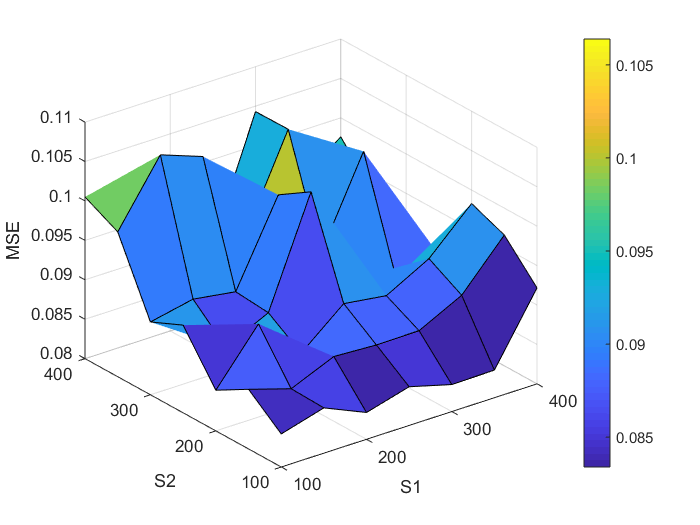
\includegraphics[width = 0.7\textwidth]{Grafika/MSE_duze.png}
\caption{Wpływ liczby neuronów w warstwie pierwszej i drugiej na błąd średnio-kwadratowy}
\label{fig:MSEeksperyment2}
\end{figure}
\clearpage
Największą poprawność klasyfikacji ($57.38\%$) uzyskano dla 250 neuronów w warstwie pierwszej i 100 w warstwie drugiej.\\
Najmniejszy błąd średnio-kwadratowy ($0.0834284$) osiągnięty został dla 300 neuronów w warstwie pierwszej i 100 neuronów w warstwie drugiej. Dla tej konfiguracji $PK$ wyniosło $54.63\%$.\\
Na podstawie powyższych obserwacji można wyciągnąć wniosek, iż duża liczba neuronów niekoniecznie wpływa pozytywnie na proces uczenia sieci. Poprawność klasyfikacji zawierała się w większości w przedziale $45-55\%$.

    \subsection{Badania przesiewowe dla średniej ilości neuronów}
Eksperyment ten miał na celu sprawdzenie jak zachowuje się sieć przy średniej ilości neuronów w dwóch warstwach. Wszystkie parametry pozostały bez zmian, zmieniana była jedynie ilość neuronów w zakresie od 10 do 100 z krokiem 10.
\begin{figure}[!h]
\centering
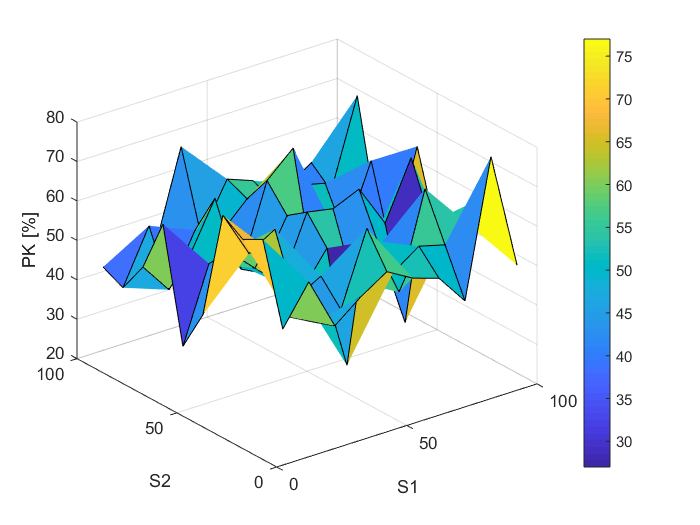
\includegraphics[width = 0.65\textwidth]{Grafika/pk_srednie.png}
\caption{Wpływ liczby neuronów w warstwie pierwszej i drugiej na poprawność klasyfikacji}
\label{fig:PKeksperyment3}
\end{figure}
\begin{figure}[!h]
\centering
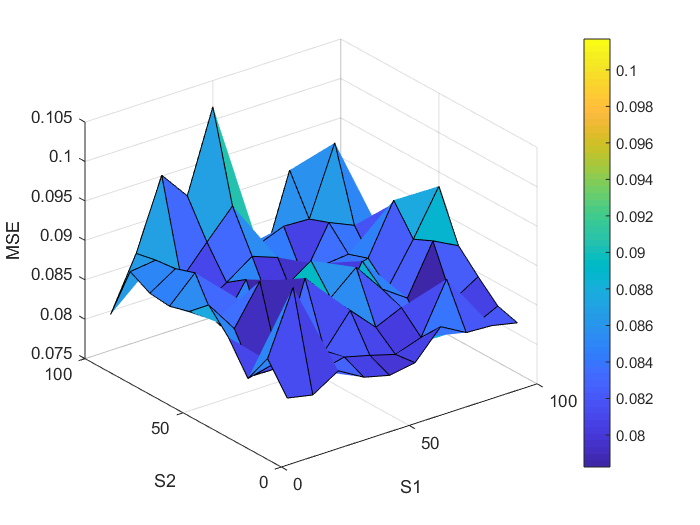
\includegraphics[width = 0.65\textwidth]{Grafika/mse_srednie.png}
\caption{Wpływ liczby neuronów w warstwie pierwszej i drugiej na błąd średnio-kwadratowy}
\label{fig:MSEeksperyment3}
\end{figure}

Największą poprawność klasyfikacji ($57.38\%$) uzyskano dla 250 neuronów w warstwie pierwszej i 100 w warstwie drugiej.\\
Najmniejszy błąd średnio-kwadratowy ($0.0834284$) osiągnięty został dla 300 neuronów w warstwie pierwszej i 100 neuronów w warstwie drugiej. Dla tej konfiguracji $PK$ wyniosło $54.63\%$.\\
    \subsection{Badania w zakresie najefektywniejszych konfiguracji neuronów}
Biorąc pod uwagę wyniki poprzednich eksperymentów oszacowano zakres neuronów, przy których sieć osiągała najlepsze wyniki. Przeprowadzono kolejne badanie w celu znalezienia najlepszej konfiguracji. Zdecydowano się by badać ilość neuronów w pierwszej warstwie w zakresie od 40 do 80 z krokiem 5 i ilość neuronów w drugiej warstwie od 5 do 30 z krokiem 1.
\begin{figure}[!h]
\centering
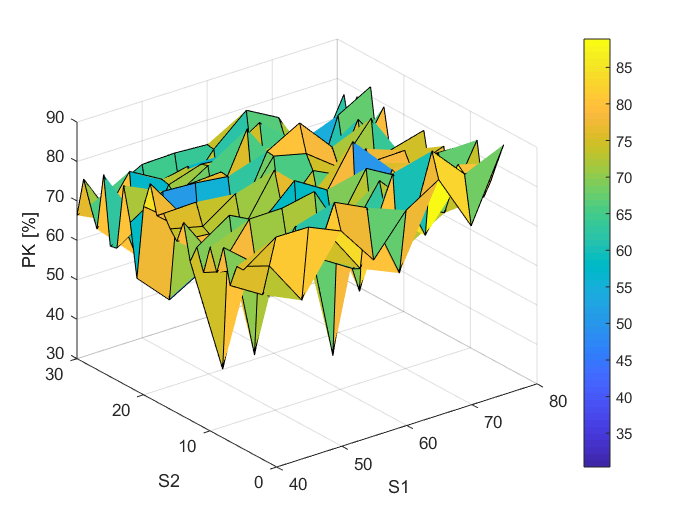
\includegraphics[width = 0.65\textwidth]{Grafika/pk4.png}
\caption{Wpływ liczby neuronów w warstwie pierwszej i drugiej na poprawność klasyfikacji}
\label{fig:PKeksperyment4}
\end{figure}
\begin{figure}[!h]
\centering
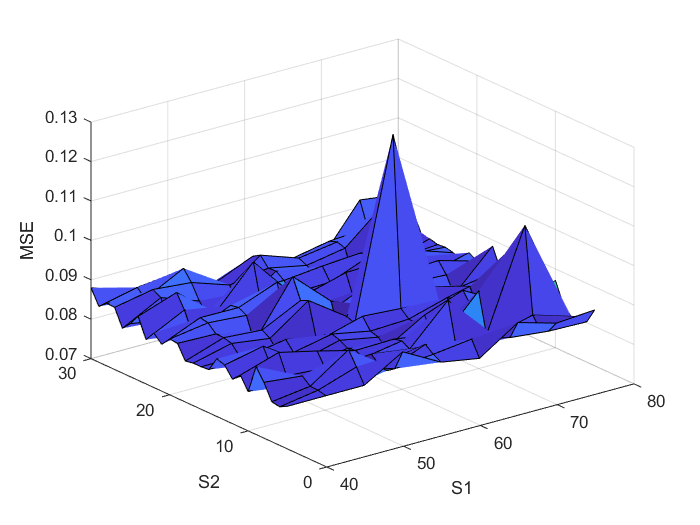
\includegraphics[width = 0.65\textwidth]{Grafika/MSE4.png}
\caption{Wpływ liczby neuronów w warstwie pierwszej i drugiej na błąd średnio-kwadratowy}
\label{fig:MSEeksperyment4}
\end{figure}

Największą poprawność klasyfikacji ($88.88\%$) uzyskano dla 70 neuronów w warstwie pierwszej i 6 w warstwie drugiej. Jednak, kilkukrotnie powtarzając te badanie nie udało się uzyskać podobnego wyniku. Średnio, najlepszą konfiguracją okazało się 70 neuronów w warstwie pierwszej i 13 neuronów w warstwie drugiej dla której większość wyników przekraczała $80\%$ poprawności klasyfikacji.\\
Najmniejszy błąd średnio-kwadratowy ($0.0766883$) osiągnięty został dla 50 neuronów w warstwie pierwszej i 8 neuronów w warstwie drugiej. Dla tej konfiguracji $PK$ wyniosło $72.13\%$.\\
    \subsection{Badania wpływu parametrów adaptacyjnych na uczenie sieci}
Na podstawie wyników poprzednich eksperymentów ustalono konfigurację sieci na 70 neuronów w warstwie pierwszej i 13 w warstwie drugiej. Współczynnik uczenia ustawiono na 0.01. Pozostałe współczynniki zmieniano w zagnieżdżonych pętlach. Współczynnik zwiększania wartości współczynnika uczenia $lr\_inc$ zmieniano w zakresie od 1.03 do 1.07 z krokiem 0.01, współczynnik $lr\_dec$ w zakresie od 0.6 do 0.8 z krokiem 0.05, oraz dopuszczalna krotność przyrostu błędu (w Matlab'ie $max\_perf\_inc$) w zakresie od 1.02 do 1.06 z krokiem 0.01.

\begin{figure}[!htb]
\minipage{0.5\textwidth}
  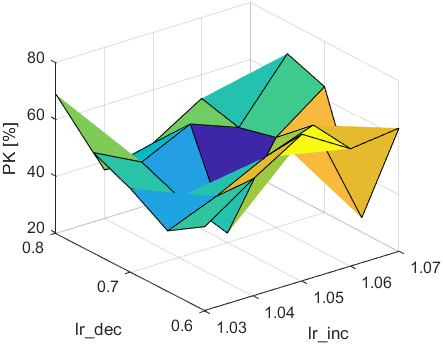
\includegraphics[width = \linewidth]{Grafika/exp5/pk102.png}
\endminipage\hfill
\minipage{0.5\textwidth}
  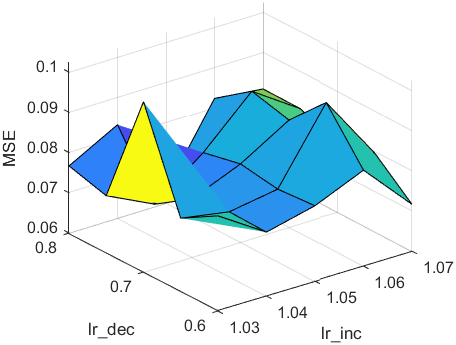
\includegraphics[width = \linewidth]{Grafika/exp5/mse102.png}
\endminipage\hfill
\caption{Wpływ $lr\_inc$ i $lr\_dec$ na $PK$ i $MSE$ dla $max\_perf\_inc=1.02$}
\end{figure}
%\\[0.5cm]
\begin{figure}[!htb]
\minipage{0.5\textwidth}
  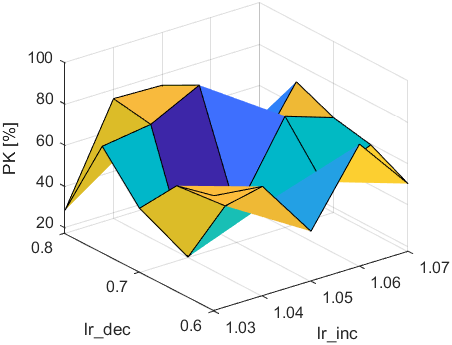
\includegraphics[width = \linewidth]{Grafika/exp5/pk103.png}
\endminipage\hfill
\minipage{0.5\textwidth}
  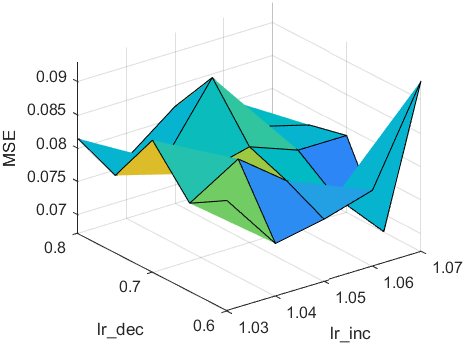
\includegraphics[width = \linewidth]{Grafika/exp5/mse103.png}
\endminipage\hfill
\caption{Wpływ $lr\_inc$ i $lr\_dec$ na $PK$ i $MSE$ dla $max\_perf\_inc=1.03$}
\end{figure}

\clearpage
\begin{figure}[!htb]
\minipage{0.5\textwidth}
  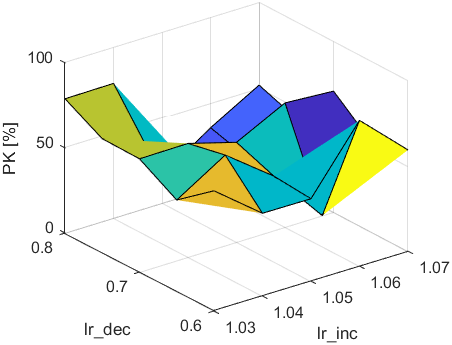
\includegraphics[width = \linewidth]{Grafika/exp5/pk104.png}
\endminipage\hfill
\minipage{0.5\textwidth}
  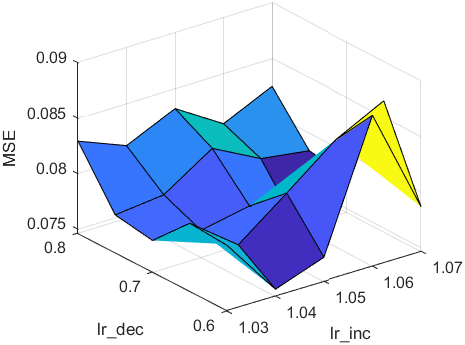
\includegraphics[width = \linewidth]{Grafika/exp5/mse104.png}
\endminipage\hfill
\caption{Wpływ $lr\_inc$ i $lr\_dec$ na $PK$ i $MSE$ dla $max\_perf\_inc=1.04$}
\end{figure}

\begin{figure}[!htb]
\minipage{0.5\textwidth}
  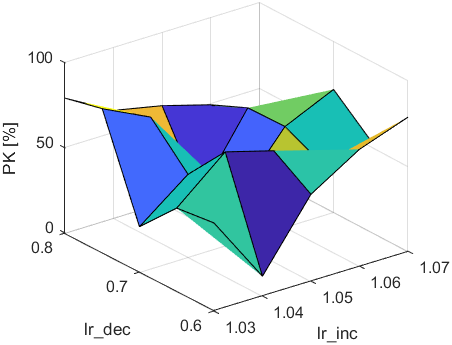
\includegraphics[width = \linewidth]{Grafika/exp5/pk105.png}
\endminipage\hfill
\minipage{0.5\textwidth}
  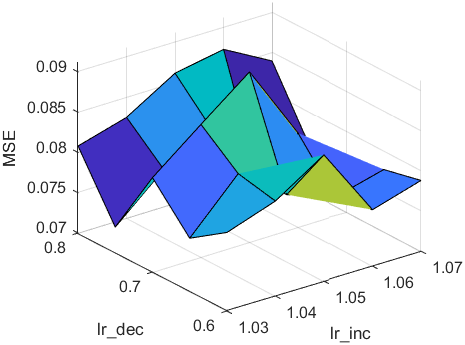
\includegraphics[width = \linewidth]{Grafika/exp5/mse105.png}
\endminipage\hfill
\caption{Wpływ $lr\_inc$ i $lr\_dec$ na $PK$ i $MSE$ dla $max\_perf\_inc=1.05$}
\end{figure}
\begin{figure}[!htb]
\minipage{0.5\textwidth}
  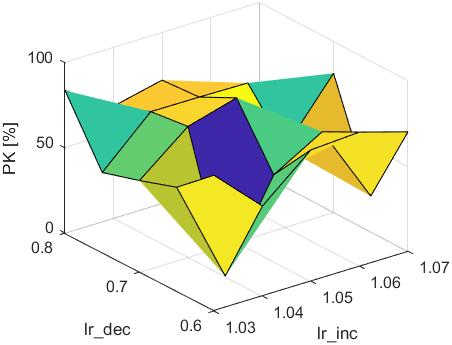
\includegraphics[width = \linewidth]{Grafika/exp5/pk106.png}
\endminipage\hfill
\minipage{0.5\textwidth}
  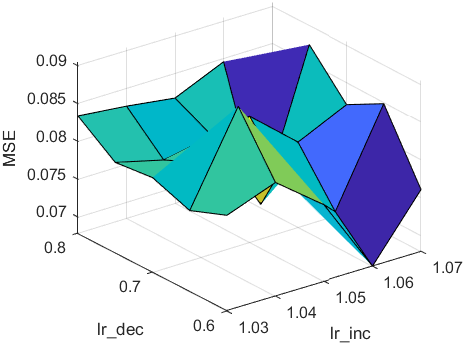
\includegraphics[width = \linewidth]{Grafika/exp5/mse106.png}
\endminipage\hfill
\caption{Wpływ $lr\_inc$ i $lr\_dec$ na $PK$ i $MSE$ dla $max\_perf\_inc=1.06$}
\end{figure}

Największą poprawność klasyfikacji ($85.63\%$) uzyskano dla $lr\_inc = 1.06$, $lr\_dec = 0.6$ i $max\_perf\_inc=1.04$. Błąd średnio kwadratowy dla tej konfiguracji wynosił $0.0882536$.
    \subsection{Sprawdzenie algorytmu na innym zbiorze danych}\label{eksperyment6}
W przeprowadzonych eksperymentach osiągane wyniki nie były zadowalające. Poprawność klasyfikacji nie przekroczyła nawet $90\%$. Aby sprawdzić czy skrypt sieci neuronowej został wykonany poprawnie, wykorzystano zbiór danych $Iris$. Jest to na tyle popularny zestaw, że znalazł swoje miejsce w domyślnych zestawach danych oprogramowania Matlab R2019a. Zbiór zawiera 3 klasy po 50 rekordów, które odnoszą się do rodzaju kwiatu irysa.\\
Przeprowadzono test dla domyślnych parametrów adaptacyjnych. Zmieniana była jedynie liczba neuronów w obu warstwach w zakresie od 10 neuronów do 70 z krokiem 10.
\begin{figure}[!h]
\centering
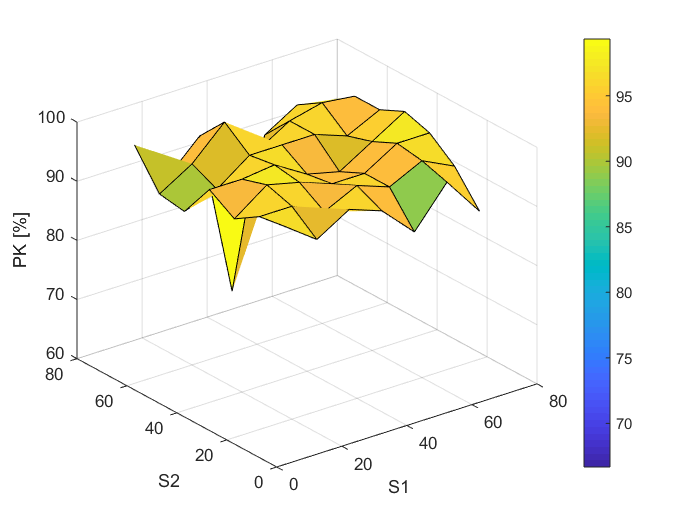
\includegraphics[width = 0.7\textwidth]{Grafika/iris_PK.png}
\caption{Wpływ liczby neuronów w warstwie pierwszej i drugiej na poprawność klasyfikacji}
\label{fig:iris_PK}
\end{figure}

Osiągnięte wyniki były zauważalnie lepsze, co potwierdza poprawność algorytmu. Dla większości konfiguracji uzyskano poprawność klasyfikacji powyżej $90\%$. Największą poprawność klasyfikacji ($99.33\%$) uzyskano dla 30 neuronów w warstwie pierwszej i 60 neuronów w warstwie drugiej.
    
    \clearpage
    \section{Wnioski}
    Projekt zakładał stworzenie skryptu realizującego sieć neuronową uczoną algorytmem wstecznej propagacji błędu z przyśpieszeniem metodą adaptacyjnego współczynnika uczenia. Dzięki oprogramowaniu Matlab jest to możliwe nawet dla osoby dopiero zaznajamiającej się z tematem sztucznej inteligencji. Pakiet Deep Learning Toolbox zawiera wiele funkcji mocno ułatwiających realizację sieci neuronowych. Istnieje nawet możliwość wygenerowania skryptu w kreatorze graficznym, co ułatwia i przyśpiesza tworzenie sieci.\\[0.2cm]
    Aczkolwiek, pełne wykorzystanie możliwości sieci neuronowych wymaga sporo wiedzy i przeprowadzania wielu eksperymentów. Szukanie odpowiednich parametrów sieci, takich jak ilość neuronów w warstwach, czy innych współczynników może zająć nawet kilkanaście godzin.\\[0.5cm]
    Wyniki eksperymentów dla zadania rozpoznawania substancji odurzających nie były satysfakcjonujące. Nie udało się osiągnąć oczekiwanej poprawności klasyfikacji bliskiej $100\%$. Należy jednak wziąć pod uwagę szczególność zestawu danych $Dorothea$. We wspomnianym zestawie znajduje się 256 różnych atrybutów przy tylko 800 przypadkach, w których 722 to wystąpienia negatywne. Jak podają autorzy zbioru, wartości niektórych z atrybutów zostały wygenerowane losowo i nie różnią się od siebie w znacznym stopniu. Możliwym jest, że sieć osiągała by wyższe wyniki poprawności klasyfikacji, gdyby zestaw danych posiadał więcej przypadków dla obu klas.\\[0.2cm]
    Poprawność wykonania algorytmu została potwierdzona w eksperymencie (\ref{eksperyment6}), gdzie zbadano jakie wyniki uda się osiągnąć sieci dla zestawu danych $Iris$ $Data$ $Set$. Osiągnięto wysoką poprawność klasyfikacji bliską $100\%$.
   
    
    
    \clearpage
    \thispagestyle{empty}
\begin{thebibliography}{9}

\bibitem{book} 
Rutkowski L.
\textit{Metody i techniki sztucznej inteligencji, Wydawnictwo Naukowe PWN, Warszawa 2019}

\bibitem{neuron} 
dr hab. inż. Roman Zajdel. 
\textit{Sztuczna inteligencja, Laboratorium, Ćw6 Model neuronu}. 
PRz.

\bibitem{siec_jednowarstwowa} 
dr hab. inż. Roman Zajdel. 
\textit{Sztuczna inteligencja, Laboratorium, Ćw8 Sieć jednokierunkowa jednowarstwowa}. 
PRz.

\bibitem{siec_wielowarstwowa} 
dr hab. inż. Roman Zajdel. 
\textit{Sztuczna inteligencja, Laboratorium, Ćw9 Sieć jednokierunkowa wielowarstwowa}. 
PRz.

\bibitem{momentum} 
dr hab. inż. Roman Zajdel. 
\textit{Sztuczna inteligencja, Laboratorium, Ćw10 Przyśpieszanie procesu uczenia}. 
PRz.

\bibitem{Kluska} 
prof. dr hab. inż. Jacek Kluska. 
\textit{Wykład o metodzie wstecznej propagacji}. 
PRz.

\bibitem{mathworks}
\url{https://www.mathworks.com/help/deeplearning/ref/traingda.html}

\bibitem{mathworks}
\url{https://archive.ics.uci.edu/ml/datasets/dorothea}

\end{thebibliography}

    \listoffigures
    %\listoftables
    \lstlistoflistings
\end{document}
    